\documentclass{bioinfo}
\copyrightyear{2010}
\pubyear{2010}

\begin{document}
\begin{application}
\firstpage{1}

\title[SMM Project]{Stabilization matrix method - Mini project}
\author[Sigmar Stefansson, Francesco Favero]{Sigmar Stefansson and Francesco Favero}
\address{Danmarks Tekniske Univeristet}

\history{22 October 2010}

\editor{Supervisor: Morten Nielsen}

\maketitle

\begin{abstract}

\section{Summary}
We look at two Stabilization matrix methods \cite{SMM} used for predicting binding affinity of immunogenic peptides to major histocompatibility complex \cite{wiki:MHC} (MHC) molecules.
The testing data available was from 35 different MHC molecules from HLA-A and HLA-B, with number of peptides ranging from 59 to 3089.

\end{abstract}

\section*{Introduction}

\section*{Material and Methods}

We were given semi-completed code for the implementation of the Stabilization matrix method. The minimization procedures were gradient descent in one case and monte carlo in the other. The testing data available was from 35 different MHC molecules from HLA-A and HLA-B, with number of peptides ranging from 59 to 3089. In addition to finishing the code we added some optimizations like skipping unnecessary memory allocations at performance critical locations. We ran the matrix creation on each 35 MHC molecules to get the broadest perspective.
The data for each MHC molecule was splitted into five parts, equally (or nearly equally) sized. Each part was then used for the validation of the model trained on the rest (4/5) of the data, resulting in 5 iterations to be used for (5-fold) cross-validation.
The lambda value controls the.



\section*{Results}



\begin{figure}[!tpb]
\centerline{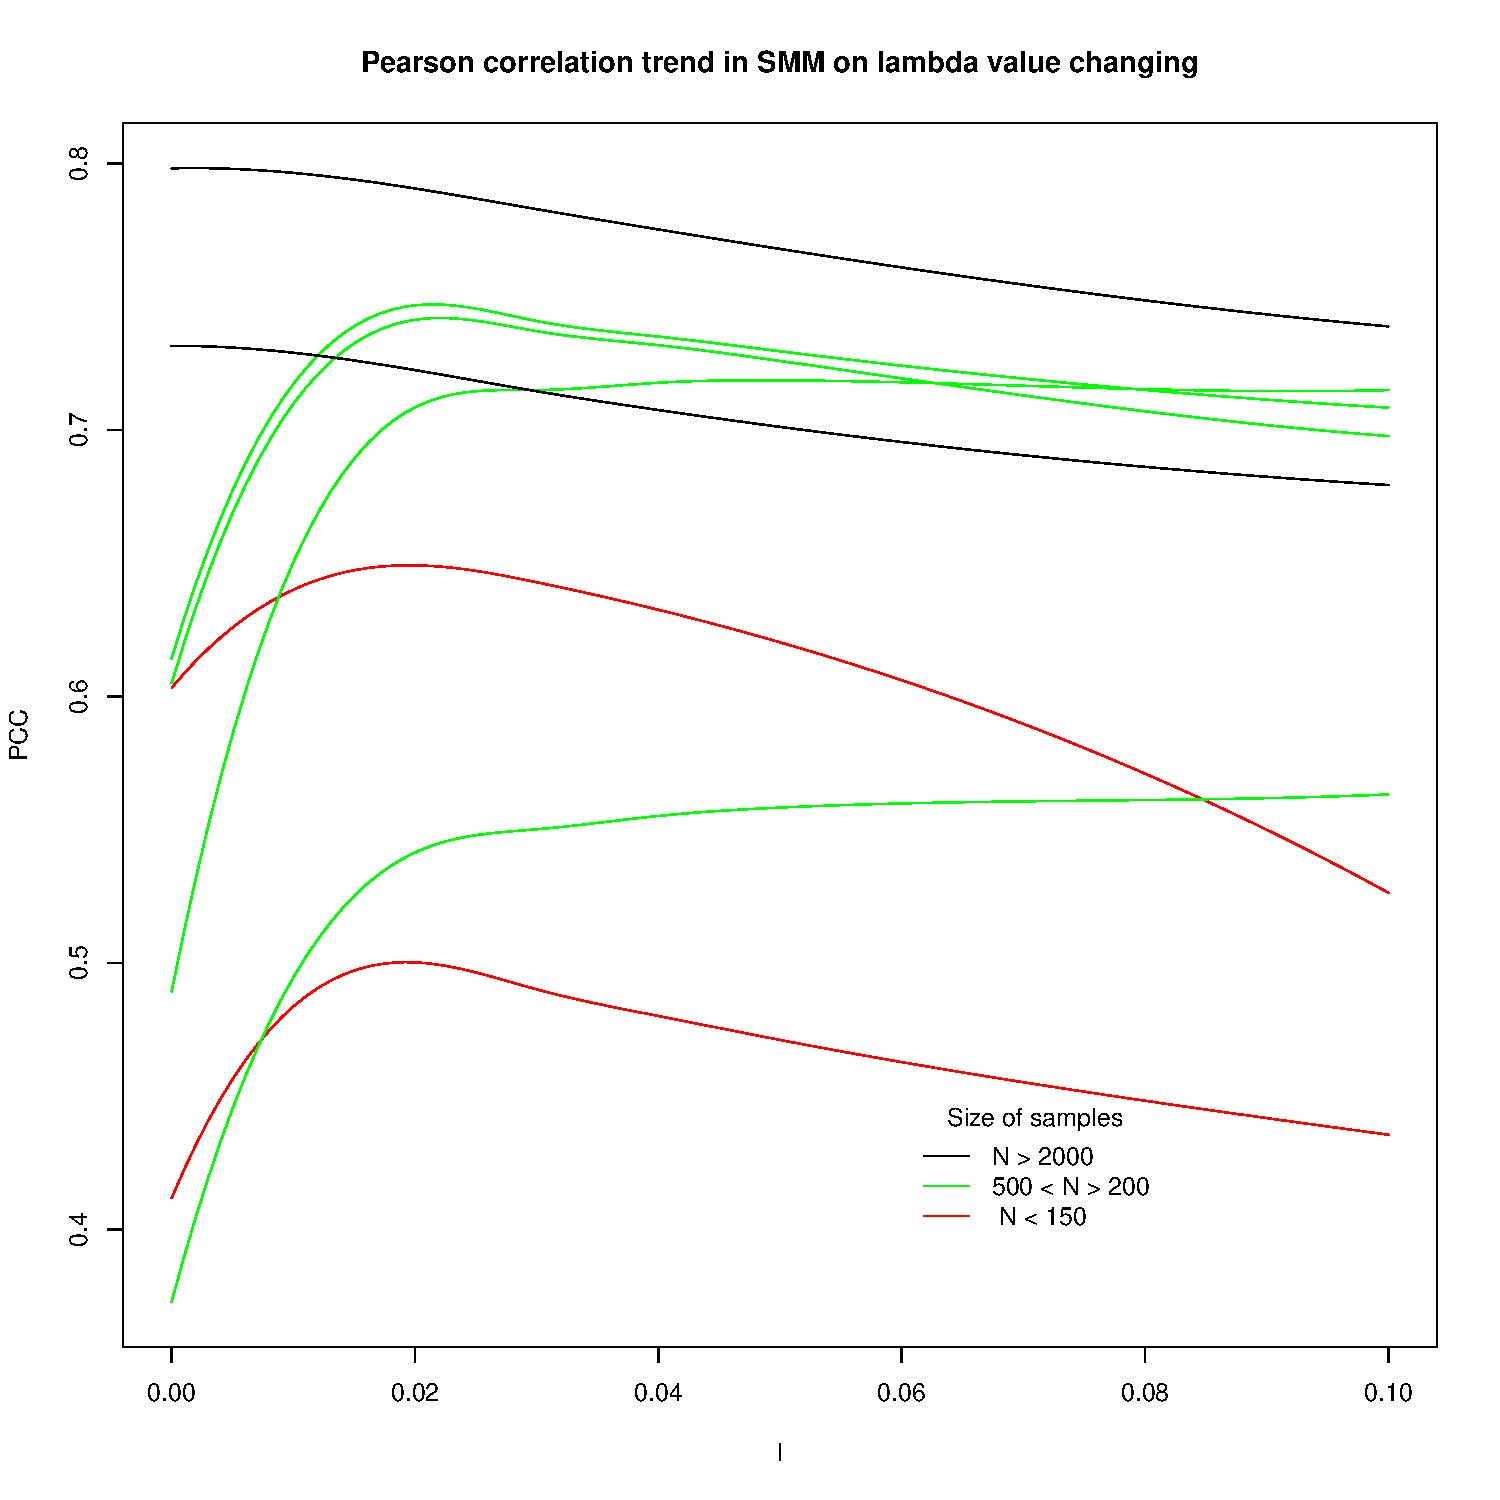
\includegraphics[width=9cm]{fig/smm_l_ppc_size.pdf}}
\caption{blablabla}\label{fig:01}
\end{figure}





%\bibliographystyle{natbib}
%\bibliographystyle{achemnat}
%\bibliographystyle{plainnat}
%\bibliographystyle{abbrv}
%\bibliographystyle{bioinformatics}

\bibliographystyle{abbrv}

\bibliography{algo}


\end{application}
\end{document}
